Testing of the program was performed in two main ways, testing of the indidual functions and testing of the system as a whole.
certain functions designed to accelerate the raytracing need to be compared to a base implementation that while slower is
guaranteed to be correct, for instance a finding the closest intersection of a ray and mesh, the simplest way to do this
is to test the ray and every triangle in the mesh and record the closest intersection, this is simple to perform and
the scope for errors in the implementation is low, unfortuanatly this is a very expensive operation that requires $\Omega(n)$
time complexity, in this project the k-d tree is used to accelerate the test, this can be performed in $\Omega(log(n))$ time
complexity, the code to perform the intersection test for this data structure is much more complicated and as a result
errors in the implementation are more likely. Testing of these complicated functions was done by comparing the output
of the simple function with the faster implementation this can be used to ensure that the outputs match, it can also be
used to see if the new implementation does indeed increase the performance of the code. Figure~\ref{fig:testing_performance_comp}

\section{System Testing}
\begin{figure}[h!]
\missingfigure{Performance Comparison}
\label{fig:testing_performance_comp}
\caption{Performance difference for triangle intersections}
\end{figure}

\subsection{Photon Viewer}
As the development of the system was performed roughly in the order described in the document, the photon map was produced before the
system used it in the radiance estimate when creating the images, as a result the result the verifiing the results of the photon
map generator posed a paticular challange as it typically contained thousands of photons in a geometry independant data structure, as
part of the development of the product we created a companion utility to the main system that allows for the visualisation of the
photon map, when inputed into the program we can see if the results match the expectation of the distribition of the photons for a
given scene. The photon viewer is reads in data from a simple format containing as a first line the number of photons and then
a list of the same length of photon positions, powers and incident directions. This tool proved to be of great value also being used
to test the sampling functions. The design of the photon viewer is simalar to that of the main GUI, differring in that it displays points
stored in an OpenGL display list \cite{khronos:2014:online}  (used to lower the number of draw calls) as oppose to rendering a
texture of the output image as in the main GUI.

\begin{figure}
\centering
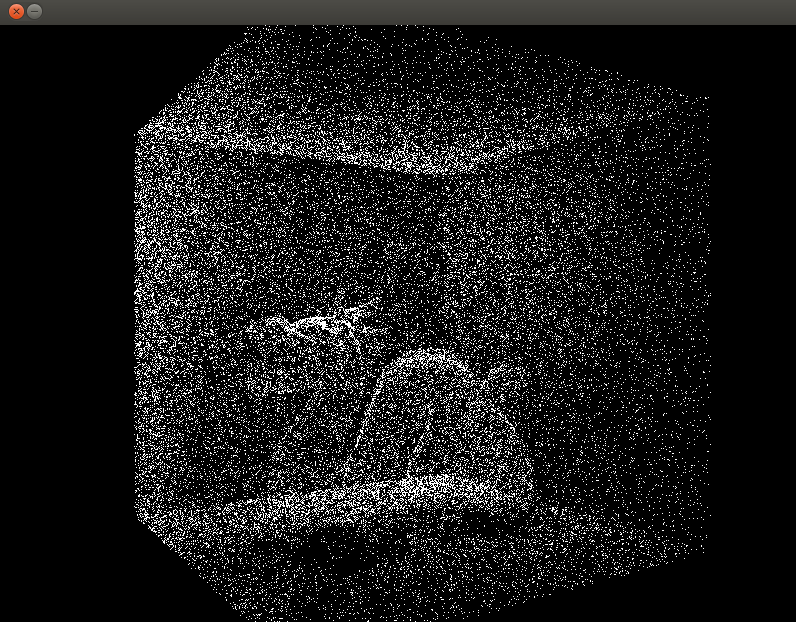
\includegraphics[width=0.7\textwidth]{./images/photon_viewer.png}
\label{fig:photon_viewer}
\caption{Photon Viewer Running}
\end{figure}

\subsection{Pixel Tracing}
When performing tests on the system it would frequenetly be the case that a change introduced obvious error in the output image,
it became apparant early in the development that being able to trace a single pixels path through the scene would make the
task of debugging that much easier. This functionallity is available as the \texttt{--trace\_pixel} option.

\section{Peformance Testing}
During the design and implementation of the system we have stated that certain descitions were made in order to improve the performance
of the system, in this section we will present results of testing that was performed in order to evaluate the gains from these descitions.

\subsection{Photon Nearest Neighbour Search}

\subsection{K-D tree intersection acceleration}

\subsection{Multicore Scaling}
In Chapter \todo{Reqs} and \todo{Design} we highlighted the inherent parralism possible in the
photon mapping algorithm in both the photon generation and raytracing stages, in order to
test the performance of the system and its ability to scale with more resources we decided to
aquire access to Amazon EC2 compute clusters, allowing us to run the system on up to 32 Intel
Xeon E5-2670 cores and 60GB of RAM \cite{amazon-instances}, we tested the system with various
settings such as resolution and number of photons in the photon map and in the radinace estimate
, each configuration will be run multiple times in order to reduce variance due to the hardware.

